\documentclass[times]{ettauth}
%\documentclass[times,doublespace]{ettauth}%For paper submission

\usepackage{acronym}
\usepackage{flafter}


\begin{document}
\newacro{gdp}[GDP]{Gross Domestic Product}
\newacro{citysdk}[CitySDK]{Smart City Service Development Kit and its application Pilots}
\newacro{W3C}[W3C]{World Wide Web Consortium}
\newacro{POI}[POI]{Point of Interest}
\newacro{XML}[XML]{Extensible Markup Language}
\newacro{JSON}[JSON]{JavaScript Object Notation}
\newacro{REST}[REST]{Representational State Transfer}
\newacro{HATEOAS}[HATEOAS]{Hypermedia as the Engine of Application State}
\newacro{poi}[POI]{Point of Interest}
\newacro{gis}[GIS]{Geographical Information System}
\newacro{wg}[WG]{Working Group}
\newacro{iptc}[IPTC]{International Press Telecommunications Council}
\newacro{POIs}[POIs]{Points of Interest}



\runningheads{P. Cruz \emph{et al}}{CitySDK Tourism API - Building value around open data}

\articletype{Research Article - CONFIRM}

\title{CitySDK Tourism API - Building value around open data}
\author{Pedro Cruz\affil{1},
Ricardo Lopes Pereira\affil{2}\affil{1}\corrauth\,
Andr\'e Oliveira\affil{3} and 
Geert Monsieur\affil{4}}
\address{
 \affilnum{1}Instituto Superior T\'ecnico, Avenida Rovisco Pais 1, 1049-001 Lisboa, Portugal\\
 \affilnum{2}INESC-ID, Av. Prof. Dr. Cavaco Silva, 2744-016 Porto Salvo, Portugal\\
 \affilnum{3}ISA\\
 \affilnum{4}Geert's address
}
\corraddr{E-mail: ricardo.pereira@inesc-id.pt}

\begin{abstract}
To be written latter.
\end{abstract}

\maketitle

\acresetall
\section{Introduction}

\subsection{Motivation}
The value of tourism as an economic and leisure activity.

The amount and quality of data that municipalities have in their information systems. 
Data is held not only by cities but by other entities as well.
Municipalities understand the value of this data and have gone through a multi-step process for sharing this data with tourists in order to improve their experience and attract them to the city.

First municipalities create apps for sharing data with the tourists.
Small market to recuperate investment.
Municipalities are not software houses: unable to keep up with the pace of innovation. 
They are limited in the types of applications they can provide: e.g. publishing negative opinions.

Then municipalities made data available to programmers through internal open data initiatives.
Each city uses its own format.
Programmers still have to deal with a small market.
Tourists still have difficulties finding the specific apps for each city.

\subsection{Challenges}
Common API when intersection among available data is small.
Flexibility to accommodate further usages not yet envisioned.

make way for delegation and common developer keys?


\subsection{CitySDK}
Talk about the project.

Briefly introduce the API.

This document is organised ...

This is an acronym expansion: \ac{citysdk}.
This is a test citation, to be removed later~\cite{1509968}.



\section{Related work}

\subsection{\acf{W3C} POI Working Group}
The \ac{W3C} is an international community where Member organizations, a full-time staff, and the public work together to develop Web standards. This community is led by Web inventor Tim Berners-Lee and CEO Jeffrey Jaffe. 

One of the its working groups is the \ac{W3C} POI~\cite{w3c-poi} and its mission is to develop technical specifications for the representation of \acf{POI} information on the Web. Its Core defines a generic, flexible, lightweight and extensible POI data model, and one normative syntax for the data model based on \acf{XML}. Although \ac{XML} is the primary model for this specification, other formats are also possible, such as \acf{JSON}.

The data model is shown in Figure~\ref{fig:data-model}. The data model is comprised of six entities:
\begin{itemize}
\item \textbf{POIBaseType} is the common entity from which the majority of POI entities are derived. It provides basic properties related with its authorship, licensing, modification times and identification and thus allowing each element to carry distinct information.
\end{itemize}

\begin{figure*}[ht]
\centering
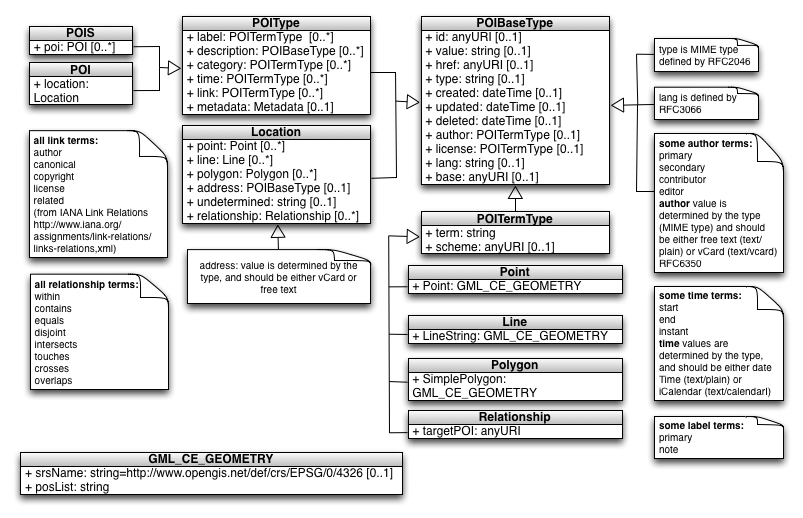
\includegraphics[width=0.8\textwidth]{images/uml.png}
\caption{W3C POI Core Data Model}
\label{fig:data-model}
\end{figure*}

opendata

tourism and POI APIs

REST APIs?


\section{API design}

\subsection{W3C POI Model in the API}
W3C POI - who it is used

\subsection{API Description}
describe the API

\subsection{Delegation}
different roles: programmer, city, museum, world wide directory.


\section{Implementation}
Talk about Lisbon's implementation



\section{Evaluation}
Answer how the challenges were met.

Evaluate the architecture from other perspectives: performance - http load balancing + delegation to multiple servers; ??



\section{Conclusions}


\acks
thank you

\bibliographystyle{wileyj}
\bibliography{references}

\end{document}


% Local IspellDict: "british"
% Local IspellPersDict: "~~/.ispell-English"

% Local Variables:
% mode: flyspell
% End:
